\chapter{Tests mit Unity}
\label{sec:Tests mit Unity}

In diesem Kapitel möchte ich untersuchen, welche Möglichkeiten es zur Zeit gibt, um seine Skripte automatisiert zu testen. Dabei zeige ich zunächst kurz, wie man sein Spiel mit dem Test-Framework der Entwicklungsumgebung testen kann. Anschließend stelle ich die Frameworks der Unity-Fangemeinde und abschließend analysiere ich die Möglichkeiten und erläutere deren Probleme.

\section{Unit Test Framework der Entwicklungsumgebung (MSTest)}

Eine Möglichkeit ist es, das Framework der Entwicklungsumgebung zu verwenden. Dies wäre in diesem Fall MSTest, welches in \textit{Visual Studio} integriert ist.\\
Hierbei ist es üblich, dass man neben dem Projekt mit dem Produktivcode ein weiteres für die Tests hat. Dadurch sind diese und das Produkt sowohl räumlich, als auch logisch voneinander getrennt.

Im Nachfolgenden wird gezeigt, wie man einen Unit-Test mit MSTest aufbaut und welche Möglichkeiten es dabei gibt.

\pagebreak
\begin{lstlisting}[caption={[Unit Test mit MSTest]Unit Test mit MSTest\\
Beispiel einer Testklasse in MSTest. Zeigt wie man ihre Testmethoden deklariert und wie sie initialisiert wird.}, label=code:UnitTestMitMSTest]
using Microsoft.VisualStudio.TestTools.UnitTesting;

namespace Test_Project {
	[TestClass]
	public class UnitTest {
		[ClassInitialize]
		public static void ClassSetUp() {
			// Code to initialize the test class
			// Is called only once BEFORE all tests
		}
		[TestInitialize]
		public void SetUp() {
			// Code to intialize the single tests
			// Is called BEFORE every test
		}
		[TestMethod]
		public void TestSomething() {
			// A test
		}			
		[TestMethod]
		public void TestSomethingOther() {
			// An other test
		}
		[TestCleanup]
		public void TearDown() {
			// Code to clean the actions of the single tests
			// Is called AFTER every test
		}
		[ClassCleanup]
		public static void ClassTearDown() {
			// Code to clean the test class
			// Is called only once AFTER all tests
		}
	}
}
\end{lstlisting}
\pagebreak

Um dem Framework zu signalisieren, dass in einer Klasse Tests vorhanden sind, braucht diese das Attribut \textit{TestClass}, welches in eckigen Klammern über dem Klassennamen angegeben wird. Die einzelnen Tests in Form von Methoden werden durch \textit{TestMethod} gekennzeichnet und dürfen nichts zurückgeben und keine Parameter erwarten. Innerhalb dieser Methoden kann man mit Hilfe der Klasse \textit{Assert} bestimmte Bedingungen festlegen, die erfüllt sein müssen. Sind sie es nicht, schlägt der Test fehl und es wird eine entsprechende Meldung angezeigt. Auch wenn eine Exception nicht gefangen wird, schlägt der Test fehl und zeigt die Nachricht der Exception an.\\
Außerdem können bestimmte Methoden vor den einzelnen Tests ausgeführt werden, um zum Beispiel benötigte Objekte zu initialisieren. Dabei unterscheidet man zwischen einem Klasseninitialisierer, der genau einmal vor dem Aufruf der ersten Testmethoden ausgeführt wird und dem Testinitialisierer, der vor jedem Aufruf einer Testmethode durchgeführt wird. Der Klasseninitialisierer muss statisch sein und wird durch das Attribut \textit{ClassInitialize} markiert. Er kann zum Beispiel genutzt werden, um eine Verbindung zu einer Datenbank aufzubauen, die von mehreren Testmethoden der Testklasse verwendet wird. Der Testinitialisierer muss mit \textit{TestInitialize} gekennzeichnet werden und könnte zum Beispiel Objekte initialisieren, die von mehreren Tests gebraucht und verändert werden. Da diese dadurch vor jedem Test neu initialisiert werden, bleiben die Tests unabhängig voneinander.\\
Entsprechend zu den Initialisierern kann man auch spezielle Methoden definieren, die nach den Tests ausgeführt werden sollen. Der Klassenbereiniger könnte die zuvor geöffnete Verbindung mit der Datenbank schließen und diese von etwaigen Testdaten befreien. Der Testbereiniger kann zum Beispiel verwendet werden, um eine Singleton-Klasse auf ihren Ursprungszustand zurückzusetzen, falls dies notwendig sein sollte.

Detailliertere Informationen über das Unit Test Framework von Microsoft erhält man auf deren MSDN-Bibliotheksseite unter \url{http://msdn.microsoft.com/de-de/library/dd264975.aspx}.

Allerdings gibt es schwerwiegende Probleme, wenn man bestimmte Unity-Klassen testen möchte. Diese werden in der Analyse weiter unter näher erläutert.

\section{UUnit}

UUnit\footnote{Weitere Informationen unter \url{http://wiki.unity3d.com/index.php?title=UUnit}} ist ein Projekt der Fangemeinde für ein rudimentäres Unit Test Framework, welches in Unity Projekten verwendet werden kann. Es wurde zunächst in \textit{Boo} geschrieben, wodurch es auch Tests in \textit{Boo} erwartet. In der neusten Version (Veröffentlicht am 21.08.2012) wurde es allerdings nach C\# portiert.
Um mit UUnit Tests ausführen zu können, muss man das Framework in sein Projekt einbinden. Da UUnit Open-Source ist kann man das gesamte Framework innerhalb des \textit{Assets}-Ordners ablegen. Alternativ könnte man das Framework auch zu einer Bibliothek kompilieren und diese als Referenz einbinden.

Testklassen von UUnit müssen von der Klasse \textit{UUnitTestCase} erben, welche die beiden virtuellen Methoden \textit{SetUp} und \textit{TearDown} zur Verfügung stellt. Diese werden vor beziehungsweise nach jeder Testmethode durchgeführt und können von den expliziten Tests überschrieben werden. Die Testmethoden werden durch das Attribut \textit{UUnitTest} gekennzeichnet und mit der Klasse \textit{UUnitAssert} können Bedingungen definiert werden, die den Test fehlschlagen lassen, sollten sie nicht erfüllt sein. Allerdings bietet diese nur sechs Arten von Bedingungen, wozu \textit{Fail}, \textit{True} und \textit{Equals} gehören. Eine \textit{NotEquals}-Bedingung gibt es zum Beispiel nicht.

Innerhalb von UUnit gibt es die Klasse \textit{UUnitTestRunner}, welche alle Tests innerhalb des Projekts ausführt und das Ergebnis ausgibt. Kopiert man die Quelldatei dieser Klasse in den Ordner \textit{Assets/Standard Assets/Editor} des Unity-Proejkt, wird sogar ein neuer Knopf in die Menüleiste der Unity SDK hinzugefügt, mit dem man alle Tests ausführen lassen kann. Möchte man die Datei nicht zu seinem Projekt hinzufügen, kann man auch folgendes Skript schreiben und einem beliebigen \textit{GameObject} anfügen.

\begin{lstlisting}[caption={[Beispiel um alle UUnit-Tests auszuführen]Beispiel um alle UUnit-Tests auszuführen\\
Muss an ein \textit{GameObject} angehängt werden, wodurch beim Start des Spiels alle Tests ausgeführt werden.}, label=code:UUnitTestRunner]
public class TestRunner : MonoBehaviour {
	public void Start() {
		UUnitTestRunner runner = new UUnitTestRunner();
		runner.RunAllTests();
	}
}
\end{lstlisting}

Die Ergebnisse des Testdurchlaufs werden auf der Konsole von Unity ausgegeben, was man in der Abbildung unten sehen kann. Dabei werden die Fehlermeldungen der fehlgeschlagenen Tests, sowie die Anzahl der durchgeführten und fehlerhaften Tests ausgegeben.

\begin{figure}[h]
\centering
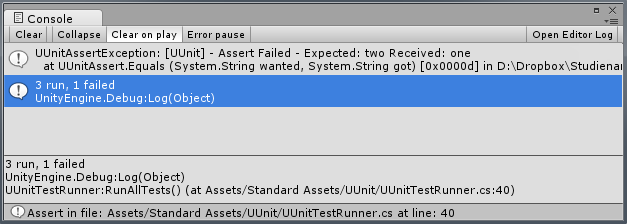
\includegraphics[width=1\linewidth]{./images/Kapitel_UnitTestsMitUnity/UUnit_Konsolenausgabe}
\caption[Ausgabe von UUnit]{Ausgabe von UUnit}
\label{fig:UUnit_Konsolenausgabe}
\end{figure}
\clearpage

\section{SharpUnit}\label{sec:SharpUnit}

SharpUnit\footnote{Weitere Informationen unter \url{http://wiki.unity3d.com/index.php?title=SharpUnit}} ist auch ein Projekt der Fangemeinde und ist in C\# implementiert. Es wurde entwickelt, da UUnit zunächst nur in \textit{Boo} zur Verfügung stand. Es orientiert sich an UUnit und hat einige Gemeinsamkeiten damit.\\
Um Tests ausführen zu können, muss man SharpUnit in sein Unity-Projekt einbinden, was wie bei UUnit funktioniert.

Testklassen müssen bei SharpUnit von der Klasse \textit{TestCase} erben, welche es ermöglicht die Methoden \textit{SetUp} und \textit{TearDown} zu überschreiben. Testmethoden werden durch das Attribut \textit{UnitTest} gekennzeichnet. Auch SharpUnit stellt einem eine Klasse zur Definition von Bedingungen zur Verfügung, wobei diese in etwa denen von UUnit entsprechen. Allerdings fehlt \textit{Fail} mit dem man einen Test geziehlt fehlschlagen lassen kann. Dafür gibt es die Möglichkeit, eine erwartete Exception zu definieren. Dies beschränkt sich allerdings auf eine pro Test, das heißt man kann keine zwei Exceptions innerhalb einer Testmethode erwarten.
 
Im Gegensatz zu UUnit können die Tests von SharpUnit nur zu Beginn des Spiels ausgeführt werden. Dafür benötigt man ein Skript, welches in der \textit{Start}-Methode bestimmte Aktionen ausführt und an ein \textit{GameObject} angehängt wird. Der nachfolgende Code ist das Beispiel von SharpUnit für so ein Skript.
\pagebreak

\begin{lstlisting}[caption={[Einbindung der Tests mit SharpUnit]Einbindung der Tests mit SharpUnit\\
Quelle: Demo von SharpUnit, erhältlich unter \url{https://github.com/mgants4/SharpUnit}.}, label=code:SharpUnitTestRunner]
public class Unity3D_TestRunner : MonoBehaviour {
	void Start() {
        // Create test suite
        TestSuite suite = new TestSuite();

        // Example: Add tests to suite
        suite.AddAll(new Dummy_Test());

        // Run the tests
        TestResult res = suite.Run(null);

        // Report results
        Unity3D_TestReporter reporter = new Unity3D_TestReporter();
        reporter.LogResults(res);
	}
}
\end{lstlisting}

Zunächst wird eine SharpUnit \textit{TestSuite} erzeugt, zu der die zu testenden Tests hinzugefügt werden. Dafür ruft man \textit{AddAll} der Suite auf und übergibt ihr eine Instanz einer Testklasse, wodurch deren Testmethoden registriert werden. Hat man die gewünschten Tests hinzugefügt, ruft man \textit{Run} der Suite auf. Diese führt die registrierten Tests aus und gibt einem Informationen über den Verlauf, in Form einer Instanz von \textit{TestResult}, zurück. Im letzten Schritt muss man einen Test-Reporter erzeugen, um damit das Ergebnis auf der Konsole der Unity SDK auszugeben. Die Ausgabe ist sehr ähnlich mit der von UUnit, zu sehen in \autoref{fig:UUnit_Konsolenausgabe}.
\pagebreak

\section{Analyse}\label{sec:Analyse}

In diesem Abschnitt werden die oben vorgestellten Frameworks bezüglich ihres Funktionsumfangs und ihrer Probleme mit Unity analysiert und verglichen. Abschließend möchte ich die meiner Meinung nach wichtigsten Kritikpunkte erläutern.

\subsection{MSTest}

Die Vorteile des von Microsoft mitgelieferten Test-Frameworks sind zahlreich. Es hat die beste \textit{Assert}-Klasse um die Bedingungen der Tests zu formulieren, da sie viele Methoden bietet. Außerdem stellt es einem als einziges die Möglichkeit zur Verfügung, einen Klasseninitialisierer/reiniger zu definieren.\\
Die Tests müssen von keiner anderen Klasse erben, sondern werden lediglich durch ein Attribut markiert. Außerdem hat man nur wenig Aufwand, um die Tests auszuführen. Das Ergebnis des Durchgangs wird nicht in der Konsole ausgegeben, sondern als Liste der einzelnen Testmethoden. Diese Liste wird in erfolgreiche, fehlgeschlagene und nicht ausgeführte Tests unterteilt. Verwendet man das Plugin \textit{Resharper} werden die Ergebnisse mit einem Baum angezeigt, was noch übersichtlicher ist.\\
Dadurch, dass MSTest unabhängig von Unity ist, sind auch die Tests unabhängig von dem Projekt. Im Gegensatz zu den anderen Frameworks, müssen sich die Tests nicht innerhalb des Unity-Projekts befinden, sondern liegen in einem separaten Projekt. Außerdem ermöglicht dies einem die Verwendung etablierter Techniken im Bereich des Testens, welche schon zu Beginn von \textit{\ref{sec:Einleitung}. \nameref{sec:Einleitung}} vorgestellt wurden.

Allerdings hat die Verwendung von MSTest auch Nachteile. Der größte ist, dass man keine Skripte - genauer gesagt keine Klassen die von \textit{MonoBehaviour} erben - testen kann, da bei deren Erzeugung eine \textit{SecurityException} auftritt, die den Test fehlschlagen lässt. Dies liegt daran, dass die \textit{MonoBehaviour} nur in einer laufenden Unity-Umgebung intialisiert werden kann. Diese lässt sich in einem Test nicht simulieren oder mocken. Um dennoch eine großflächige Abdeckung durch Tests zu erreichen, muss man die Struktur seines Projekts stark anpassen, sodass die Skripte möglichst wenig Logik enthalten. Sie müsste in eigene Klassen ausgelagert werden, wodurch sie unabhängig von Unity testbar sind. Diese Anpassung lohnt sich nur bei neuen Projekten und auch nur wenn sich das Verhalten der Objekte sinnvoll auslagern lässt. Bei einem Shooter, dessen Spielgefühl stark von einer guten Reaktion auf Benutzereingaben abhängt, ist das zum Beispiel nur schlecht möglich, da sich diese Reaktionen nicht wirklich durch einen fest definierten Test bestimmen lassen. Und auch einem speziell für diesen Fall entwickelten Projekt (dessen Prototyp im Rahmen von \cite{TDGD13} entwickelt wurde) beträgt die Abdeckung durch die Tests lediglich 45\%. Die ausgelagerte Logik hingegen erreicht eine Abdeckung von 85\%, was zeigt, dass auch bei einem Projekt bei dem sich die Logik gut auslagern lässt viel Arbeit durch die Skripte geleistet werden muss.

Was man beim Testen eines Unity-Projekts mit MSTest beachten sollte und welche Erkenntnisse dabei gewonnen wurden lässt sich in \cite{TDGD13} nachlesen.

\subsection{UUnit und SharpUnit}

Da sich diese beiden Frameworks sehr ähnlich sind, möchte ich diese gemeinsam betrachten. Der Vorteil gegenüber MSTest besteht darin, dass man auch Skripte automatisiert testen kann, da sie direkt in das Spiel eingebunden werden und somit innerhalb der Unity-Umgebung ablaufen. Allerdings benötigt man dafür ein Skript, welches für die Ausführung der Tests zuständig ist und für das ein geringer Arbeitsaufwand anfällt (s. \autoref{code:SharpUnitTestRunner} \nameref{code:SharpUnitTestRunner}). UUnit erleichtert einem das, da man über einen Menü-Punkt der Unity-SDK alle Tests ausführen lassen kann.

Dennoch kommen beide Frameworks vom Funktionsumfang nicht an MSTest heran. Hinsichtlich der Präsentation der Ergebnisse, werden diese lediglich auf der Unity Debug-Konsole ausgegeben, was bei vielen Tests schnell unübersichtlich werden kann. Außerdem gibt es keine Möglichkeit von den Testergebnissen zu der Quelldatei des Tests springen. Ein weiterer Nachteil ist, dass die Tests nun ein Teil des Unity-Projekts sind, was man bei der finalen Versionen beachten sollte, damit die Testklassen und Testszenen nicht mit ausgeliefert werden.

Eine große Einschränkung der beiden Frameworks ist, dass man nur zum Start des Spiels testen kann, da die Definition, welche Tests durchgeführt werden soll und deren Ausführung in der \textit{Start}-Methode des Skripts erfolgt. Diesen Code in die \textit{Update}-Methode auszulagern ergibt keinen Sinn, da es keine Möglichkeit gibt den Tests einen anderen Kontext zuzuordnen. Stattdessen würde die Verlagern zur Folge haben, dass die Tests bei jeder Berechnung eines Frames durchgeführt werden.

Von daher lässt sich mit den Frameworks zwar testen, dass die Skripte korrekt erstellt werden, ihre Methoden funktionieren und man ihre Attribute nicht mit unerlaubten Werten füllt. Allerdings sind Integrations- und Akzeptanztests in einem laufenden Spiel nicht möglich.

\subsection{Zusammenfassung und Kritikpunkte}

MSTest bietet von allen Frameworks die meisten Funktionalitäten und hat selbstverständlich die beste Architektur. Allerdings lassen sich damit keine Skripte oder andere Komponenten, die eine laufende Unity-Umgebung benötigen, testen. Für alles andere ist es sehr empfehlenswert.

UUnit und SharpUnit stellen einen Ansatz dar, um Skripte zu testen, aber auch nicht mehr. Die Hauptkritikpunkte sind meiner Meinung nach:
\begin{itemize}
\item \textbf{Der Aufwand zum Ausführen der Tests}\\
Dass man die auszuführenden Tests definieren muss ist kein Problem. Allerdings finde ich es unnötig, dass der Anwender die Testergebnisse selbst ausgeben muss. Ideal wäre es, wenn man nicht einmal mehr ein Skript und \textit{GameObject} zum testen benötigen würde.
\item \textbf{Fehlender Komfort der Darstellung der Ergebnisse}\\
Eine Ausgabe auf der Konsole ist nicht sehr übersichtlich und es gibt keine Möglichkeit direkt zum Fehler zu springen. Wünschenswert wäre eine Strukturierung nach Namensraum und Klasse.
\item \textbf{Geringe Auswahl an Bedingungen (\textit{Assertions})}\\
Die \textit{Assert}-Klasse bietet nur sehr wenige Methoden, um Bedingungen zu definieren. Dieses Problem lässt sich jedoch relativ leicht durch die Verwendung von \textit{NHamcrest}\footnote{\textit{NHamcrest} ist eine Bibliothek, welche einem sehr viele Assertions bietet. Es ist eine .NET-Umsetzung des in Java geschriebenen Projekts \textit{Hamcrest}. Weitere Informationen unter \url{https://github.com/grahamrhay/NHamcrest/wiki}} beheben. Allerdings werden dadurch alle fehlschlagenden Tests als Error und nicht als Fehler eingestuft, da die geworfene Exception nicht der \textit{AssertException} der Frameworks entspricht.
\item \textbf{Es sind nur simple Tests möglich}\\
Während die anderen Punkte eher kosmetischer Natur sind, stellt dieser ein echtes Problem dar, da dadurch die möglichen Tests stark eingeschränkt werden. Eine Beseitigung dieses Problems für die gegebenen Frameworks ist nicht trivial.
\end{itemize}

Im nachfolgenden gilt es nun, möglichst viele dieser Kritikpunkte zu beseitigen.